\section{Das elastische Netz}
\label{modell}
\thispagestyle{plain}

Um die Entwicklung von Orientierungs-- oder Okulardominanzkarten mittels
aktivitätsabhängiger Selbstorganisation zu beschreiben wurde eine
Vielzahl von Modellen vorgeschlagen.  Das Gros der Studien dient der
Untersuchung von Mechanismen, die eine Entwicklung organisierter rezeptiver
Felder aus einer realtiv undifferenzierten Anfangssituation erklären
können. Hebb'sche Mechanismen allein können bereits spontane
Strukturbildung durch Symmetriebrechung bewirken \cite{linsker:1986}.  So
kann z.B. auch die Entstehung orientierungsselektiver, corticaler Zellen
durch Hebb'sche Kompetition zwischen OFF-- und ON--Eingängen beschrieben
werden~\cite{miller:1994}.

Aus vielen Deprivationsexperimenten (siehe Abschn.~\ref{plastizitaet}) ist
bekannt, daß die den visuellen Karten unterliegende Struktur der
geniculo--corticalen Projektion innerhalb einer kritischen Phase in einem
plastischen Zustand verbleibt.  Die Dauer dieser kritischen Phase liegt bei
mehreren Monaten \cite{hubel:1970}.  Neuere Untersuchungen zeigen, daß
diese Periode lang im Vergleich zu der primären Entstehung der Karten
ist. Sowohl in der Katze als auch im Affen ist die Orientierungskarte schon
eine Woche nach Augenöffnung etabliert
\cite{bonhoeffer:1995,blasdel:1995}.  Es ist daher plausibel, die auf
dieser Projektion basierenden Reizrepräsentationen in adulten Tieren am
Ende der kritischen Phase als stabilen Gleichgewichtszustand fortlaufender
Auf-- und Abbauprozesse zu betrachten.

Von den bislang vorgeschlagenen Modellen sind einzig die Vertreter der
Modellklasse der sogenannten \emph{neuronalen Merkmalskarten} in der Lage,
das Ergebnis eines solchen Prozesses zu beschreiben. Die resultierende
Karte ist hier Fixpunkt einer nichtlinearen Dynamik.  Interessanterweise
sind die Modelle aus dieser Klasse bis heute auch die einzigen, die das in
Abschnitt~\ref{90grad} beschriebene, geometrische Verhältnis zwischen
Iso--Orientierungslinien und OD--Grenzlinien korrekt reproduzieren können
\parencite[vgl. Abb.~\ref{odop_hist},links und ][]{erwin:1995}.

Im folgenden untersuchen wir den von \textcite{durbin:1991}
vorgeschlagenen Vertreter dieser Modellklasse, das sogenannte
\emph{elastische Netz}. \textcite{durbin:1987} haben diesen Algorithmus,
der auf dem von \textcite{marlsburg:1976} vorgeschlagenen ``tea
trade model'' basiert, zuerst auf die Lösung des
NP--harten Optimierungsproblems des Handlungsreisenden angewandt.

Das elastische Netz beschreibt die Dynamik von Vektoren $\mathbf{R(x)}$ ---
die sich als rezeptive Felder interpretieren lassen --- in einem abstrakten
Reizraum $\cal S$.  Jeder dieser Vektoren gehört zu einem
Neuron~$\mathbf{x}$ auf einer zweidimensionalen Cortexschicht~$\cal T$.
Die neuronale Karte zu einem bestimmten Zeitpunkt~$t$ ist durch die
Konfiguration aller Merkmalsvektoren $\mathbf{R(x)}$ zu diesem Zeitpunkt
gegeben.  Die Anpassung der Merkmalsvektoren $\mathbf{R(x)}$ an die sie
aktivierenden Stimuli $\mathbf{S}$ wird durch die Gleichung

\begin{equation}
\delta\mathbf{R(x)}=\epsilon\left[\mathbf{S-R(x)}\right]
e(\mathbf{x})\;+\;\eta\Delta \mathbf{R(x)}
\label{lernschritt}
\end{equation}

beschrieben, wobei $\epsilon$ die Lernschrittweite und $e(\mathbf{x})$ die
Erregunsantwort auf die Reize $\mathbf{S}$ darstellt.  Der zweite Term der
Lernregel~\eqref{lernschritt} erzwingt dabei die Nachbarschaftserhaltung im
Zielareal~$\cal T$ ($\Delta$ ist der Laplace--Operator in zwei
Dimensionen): benachbarte Neurone tendieren dazu, ähnliche rezeptive
Felder auszubilden. Der Parameter $\eta$ bestimmt die Stärke des
Nachbarschaftsterms.

Diese Lernregel verschiebt die rezeptiven Felder der durch $e(\mathbf{x})$
erregten Neurone in Richtung des präsentierten Reizes. Die rezeptiven
Felder dieser Neurone werden dadurch den sie erregenden Reizen ähnlicher.
Die Erregungsfunktion

\begin{equation}
e(\mathbf{x|S,R})=\frac{\exp\left(-[\mathbf{S-R(x)}]^2/2\sigma^2\right)}
{\int_{\cal
T}\!d\mathbf{x}^\prime\;\exp\left(-[\mathbf{S-R(\mathbf{x}^\prime)}]^2/2
\sigma^2\right)}
\label{erregungsfunktion}
\end{equation}

\noindent bestimmt das Gebiet der Neurone in der Cortexschicht, die auf den
präsentierten Stimulus $\mathbf{S}$ antworten, und die Größe ihrer
Erregung.  Sie beschreibt den ``weichen Wettbewerb'' im elastischen Netz:
alle Neurone, die innerhalb des Erregungsgebietes liegen, nehmen anteilig
des Ausmaßes ihrer Erregung am Lernschritt teil.  Die Normierung
in~\eqref{erregungsfunktion} beschränkt die Gesamterregung in der
Cortexschicht~$\cal T$, und erzwingt die Konkurrenz der
Neurone~$\mathbf{x}$ um die Reize~$\mathbf{S}$.  Der Parameter $\sigma$
bestimmt die Größe des Gebietes im Reizraum, durch das eine einzelne
Zelle erregt wird und dadurch indirekt die Größe eines, durch einen
einzelnen Stimulus hervorgerufenen Erregungsgebietes in der simulierten
Cortexschicht.  In der Näherung kleiner Lernschrittweiten~$\epsilon$ und
vieler Stimuli~$\mathbf{S}$ läßt sich die Dynamik des elastischen Netzes
durch die nichtlineare Integro--Differentialgleichung

\begin{eqnarray}
\frac{\partial}{\partial t}\, \mathbf{R(x)} &=&\int\limits_{\cal
S}\!\!d\mathbf{S}\; \rho(\mathbf{S})\; [\mathbf{S-R(x)}]\;
\frac{\exp\left(-[\mathbf{S-R(x)}]^2/2\sigma^2\right)}{\int_{\cal T}
\!d\mathbf{x}^\prime\; \exp\left(-[\mathbf{S-R(\mathbf{x}^\prime)}]^2/2\sigma^2\right)}\;\nonumber\\
&&+\;\eta\,\Delta\mathbf{R(x)}
\label{endyn}
\end{eqnarray}

beschreiben. Diese Kontinuumsformulierung ermöglicht einen analytischen
Zugang zu den Musterbildungsmechnismen dieses Modells
(vgl. Abschnitt~\ref{stabilitaet}).  In der Dynamik~\eqref{endyn}
bezeichnet $\rho(\mathbf{S})$ die Wahrscheinlichkeitsdichte der
Reizverteilung. Das elastische Netz minimiert die Energiefunktion

\begin{equation}
E=-\; \sigma^2\!\!\int\limits_{\cal S}\!\!d\mathbf{S}\; \rho(\mathbf{S})\;
\ln\!\!\int\limits_{\cal T}\!\!d\mathbf{x}^\prime\;
\text{e}^{-\frac{[\mathbf{S-R(\mathbf{x}^\prime)}]^2}{2\sigma^2}}+\;
\frac{\eta}{2}\!\int\limits_{\cal T}\!\!d\mathbf{x}^\prime\;
\left(\nabla\mathbf{R(\mathbf{x}^\prime)}\right)^2.
\label{energie}
\end{equation}

Sie ist, da $(\mathbf{S,R})$ auf einen endlichen Bereich des $\mathbb{R}^n$
fallen, nach unten beschränkt und garantiert somit die Existenz eines
Fixpunktes der Dynamik~\eqref{endyn}.  Für die Untersuchung der
koordinierten Entwicklung visueller Reizrepräsentationen verwenden wir die
folgende Darstellung für die RF--Parameter einer Zelle:

\begin{equation*}
\mathbf{R(x)} = \bigl[R_x(\mathbf{x}),\, R_y(\mathbf{x}),\,
r\cos(2\phi(\mathbf{x})),\, r\sin(2\phi(\mathbf{x})),\, o(\mathbf{x})\bigr]
\end{equation*}

Das Antwortverhalten einer Zelle an einem Ort $\mathbf{x}$ in der
simulierten, zweidimensionalen Cortexschicht $\cal T$ wird durch
fünf abstrakte Merkmale beschrieben: \emph{Position} ($R_x,R_y$) des
rezeptiven Feldes im visuellen Feld, \emph{Orientierungsselektivität}
($r$), \emph{bevorzugte Orientierung} ($\phi$) und \emph{Okulardominanz}
($o$).  Der abstrakte Reizraum ${\cal S}$ ist folglich eine Teilmenge
des $\mathbb{R}^5$.

\subsection{Stabilitätsanalyse}
\label{stabilitaet}

Die Dynamik des elastischen Netzes besitzt eine einfache, homogene Lösung
$\mathbf{R}_0(\mathbf{x}) = (x,\, y,\, 0,\, 0,\, 0) $. Dieser Zustand ist
gekennzeichnet durch die Abwesenheit kolumnärer Strukturen: Alle Neurone
sind binokular und zeigen keine Orientierungsselektivität. Die spontane
Strukturbildung in den kolumnären Dimensionen wird von der Stabilität
dieser homogenen Lösung in Bezug auf räumlich periodische Störungen
$\boldsymbol{\delta}(\mathbf{x}) = \mathbf{R(x)}-\mathbf{R}_0(\mathbf{x})$
bestimmt.  \textcite{hohenstein:1994} führte eine lineare
Stabilitätsanalyse des elastischen Netzes für ${\cal
S}\subset\mathbb{R}^2$ und ${\cal T}=\mathbb{R}$ durch.  Für den
vorliegenden Fall ( ${\cal S}\subset\mathbb{R}^5$ und ${\cal
T}=\mathbb{R}^2$) ergibt sich für die linearisierte Dynamik von
$\boldsymbol{\delta}(\mathbf{x})$

\begin{small}
\begin{eqnarray*}
\frac{\partial}{\partial t}\, \mathbf{\boldsymbol{\delta}(x)} &=&
-\int\limits_{\cal S}\!\!d\mathbf{S}\; \rho(\mathbf{S})\;
e^{-\frac{[\mathbf{S-R_0(x)}]^2}{2\sigma^2}}\;
\biggl\{\mathbf{\boldsymbol{\delta}(x)}\biggr.+\frac{1}{\sigma^2}
[\mathbf{S-R_0(x)}]\, \pmb{\Bigl<}\!\left[\mathbf{S-R_0(x)}\right]\pmb{\Big|\,
\delta}\mathbf{(x)}\pmb{\Bigr>}\nonumber\\
&&\qquad-\frac{1}{\sigma^2}\frac{[\mathbf{S-R_0(x)}]}{\text{I}\mathbf{(S)}^2}
\biggl.\int\limits_{\mathbb{R}^2}\!\!d\mathbf{x}^\prime\;
e^{-\frac{[\mathbf{S-R_0(\mathbf{x}^\prime)}]^2}{2\sigma^2}}\,
\pmb{\Bigl<}\!\left[\mathbf{S-R_0(\mathbf{x}^\prime)}\right]\pmb{\Big|\,
\delta}\mathbf{(\mathbf{x}^\prime)}\pmb{\Bigr>}\biggr\}\; +\; \ldots\nonumber\\ &&+\;
\eta\Delta\mathbf{\boldsymbol{\delta}(x)}\qquad\qquad
\label{lindyn}
\end{eqnarray*}
\end{small}

\noindent mit $\text{I}\mathbf{(S)} = 2\pi \sigma^2 \prod_{i=3}^5
\exp\left({-\frac{S_i^2}{2\sigma^2}}\right)$; $\pmb{\left<\cdot|\cdot\right>}$ bezeichnet
das Skalarprodukt in $\mathbb{R}^5$.  Für die kolumnären Dimensionen
($i=3,4,5$) erhält man durch Lösen der Integrale

%\begin{small}
\begin{eqnarray*}
\frac{\partial}{\partial t}\, \delta_i(\mathbf{x}) &=& -\delta_i(\mathbf{x})
+\frac{\left<S_i^2\right>}{\sigma^2}\delta_i(\mathbf{x})-\frac{\left<S_i^2
\right>}{2\pi \sigma^2}\int\limits_{\mathbb{R}^2}\!\!d\mathbf{x}^\prime\;
e^{-\frac{\mathbf{(x-x^\prime)}^2}{4\sigma^2}}\delta_i(\mathbf{x}^\prime)\nonumber\\
&& +\; \eta\Delta\delta_i(\mathbf{x}).
\end{eqnarray*}
%\end{small}

In diese linearisierte Dynamik gehen nur noch die Varianzen
$\left<S_i^2\right>$ der Reizverteilung $\rho(\mathbf{S})$ ein.  Da die
Dynamik~\eqref{endyn} translationsinvariant ist, wird der linearisierte
Integraloperator in Fourierdarstellung diagonal.  Man erhält

%\begin{small}
\begin{eqnarray*}
\frac{\partial}{\partial t}\,
\Tilde{\delta}_i(\mathbf{k})&=& \lambda_i(k)\;
\Tilde{\mathbf{\delta}_i}(\mathbf{k})\\
\text{mit}\quad\lambda_i(k)&=&\left(-1+\frac{\left<S_i^2\right>}{\sigma^2}-
\frac{\left<S_i^2\right>}{\sigma^2}\; e^{-k^2\sigma^2}-\eta
k^2\right)\nonumber
\end{eqnarray*}
%\end{small}

Die Eigenwerte $\lambda_i(k)$ bestimmen die Stabilität der homogenen
Lösung bezüglich einer Störung mit Wellenzahl $k = |\mathbf{k}|$ (und
Wellenlänge $\Lambda = 2 \pi / k$).  Alle Störungen, bei deren Wellenzahl
$k$ der zugehörige Eigenwert $\lambda_i(k)$ negativ ist, zerfallen exponentiell: die homogene Lösung
bleibt stabil. Die Störungen, zu deren Wellenzahl $k$ ein positiver
Eigenwert gehört, werden vertstärkt: Es bildet sich Struktur in den
entsprechenden Dimensionen. $\lambda_i (k)$ hat genau ein Maximum bei

\begin{equation}
k_{max}=\frac{1}{\sigma} \sqrt{\ln(\left<S_i^2\right>/\eta)}
\label{kkrit}
\end{equation}

\noindent (siehe Abb.~\ref{spektrum}a). Das Maximum ist positiv für alle
$\sigma <\sigma^\ast$, wobei

\begin{equation}
\sigma^\ast_i=\sqrt{\left<S_i^2\right>-\eta-\eta \ln(\left<S_i^2\right>/\eta)}.
\label{sigkrit}
\end{equation}

\begin{figure}[t]
\centering
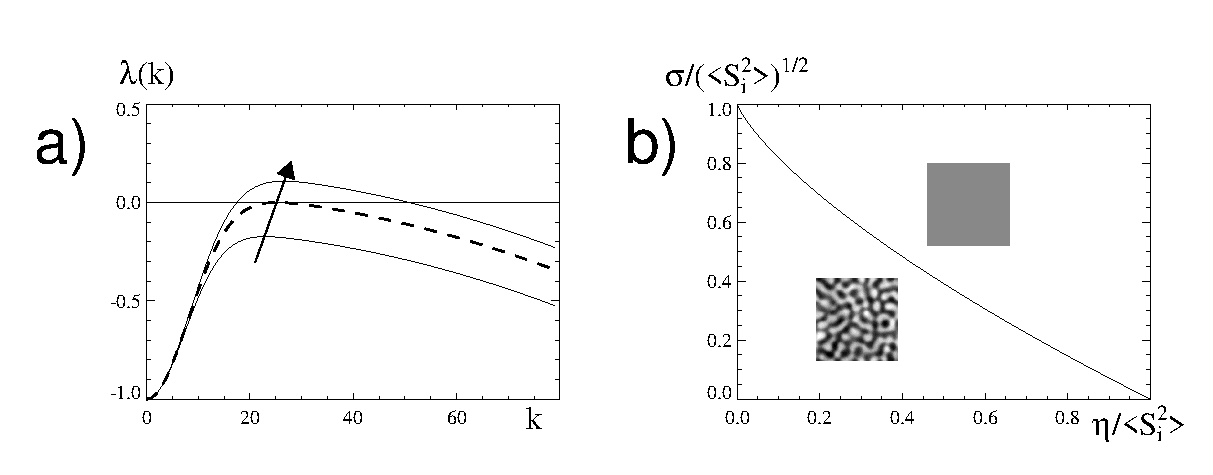
\epsfig{file=pics/analysis.eps,width=\textwidth}
\caption{\textbf{a)} Eigenwertspektrum $\lambda(k)$
der linearisierten Dynamik für verschiedene Werte von
$\sigma$ (der Pfeil skizziert die Richtung wachsenden $\sigma$'s). Die
gestrichelte Linie zeigt das Spektrum für $\sigma=\sigma^\ast$.
\textbf{b)} Phasendiagram des elastischen Netzes: Die Linie
trennt die Gebiete, in denen jeweils nur homogene bzw.  inhomogene
Lösungen stabil sind.}
\label{spektrum}
\end{figure}

Abbildung~\ref{spektrum}b zeigt, daß der durch die beiden
Parameter $\sigma$ und $\eta$ aufgespannte Phasenraum des elastischen
Netzes in zwei Gebiete zerfällt: Oberhalb der Kurve
$\sigma^\ast(\eta_{\text{rel}}),\;\text{mit}\;
\eta_{\text{rel}}=\eta/\left<S_i^2\right>$ ist die homogene Lösung,
unterhalb der Kurve  sind inhomogene Lösungen der Dynamik stabil.
Häufig wird in Simulationen der Dynamik~\eqref{endyn} der Parameter
$\sigma$ kontinuierlich verkleinert. Da $\sigma$ in der
Potentialgleichung~\eqref{energie} als Temperatur aufgefaßt werden kann,
bezeichnet man diese Vorgehensweise  auch als ``annealing''; sie
gewährleistet, daß der resultierende Endzustand optimal auf groben und
feinen Skalen ist.

Unter der Annahme fallenden $\sigma$'s ist die Wellenzahl einer kolumnären
Struktur für ein vorgegebenes, festes $\eta$ eine Funktion der
Stimulusvarianz $\left<S_i^2\right>$:

\begin{equation}
k_i^\ast = \sqrt{\frac{\ln\left(\left<S_i^2\right>/\eta\right)}{\left<S_i^2
\right>-\eta-\eta\ln\left(\left<S_i^2\right>/\eta\right)} }
\label{k_of_var}
\end{equation}

Über diese Beziehung sind die Wellenlängen der entstehenden Strukturen an die
kritischen Kooperationsreichweiten $\sigma^\ast_i$ gekoppelt.  Die
Wellenlängen der entstehenden kolumnären Strukturen sind in diesem
Fall über die Varianzen $\left<S_i^2\right>$ determiniert.  Die Analyse
zeigt damit, daß die Dynamik des
elastischen Netzes   kritisch von $\sigma$ abhängt. Für jede
kolumnäre Dimension existiert eine individuelle, kritische
Kooperationsreichweite $\sigma^\ast_i$, die unterschritten werden muß
damit sich kolumnäre Strukturen ausbilden.

\subsection{Phasenübergang}

\begin{figure}[t]
\centering
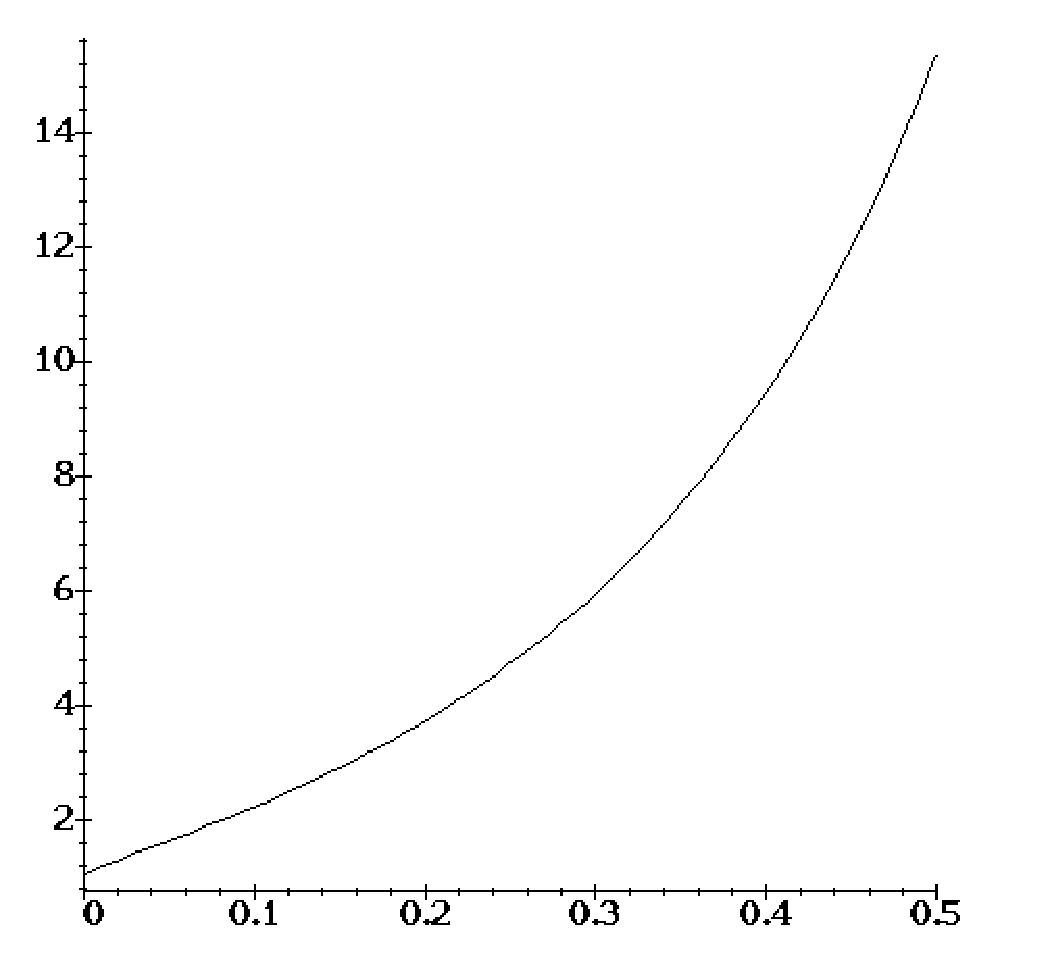
\epsfig{file=pics/koeffizient.eps,width=7cm}
\caption{Der Koeffizient des vierten Gliedes der Taylorentwicklung von
$E=E(A,\eta,\sigma)$ um $A$ ist eine monoton
wachsende Funktion, die bei 1 divergiert.}
\label{koeffizient}
\end{figure}

Zur Untersuchung der Frage, von welche Art der Übergang von homogenen zu
inhomogenen Lösungen an der Phasengrenze $\sigma^\ast(\eta_{\text{rel}})$
ist untersuchen wir die Energie für die einfachste Konfiguration von $\cal
S$ und $\cal T$ mit ${\cal S} =\mathbb{R}^2$ und ${\cal T}=\mathbb{R}$. Zur
Näherung der Lösung in Nähe des kritischen Punktes betrachten wir den
Ansatz:

\begin{eqnarray}
\mathbf{R}_A(x)&=&{\binom{x}{A\cos(k_{\text{max}}\,x)}}
\label{ansatz}
\end{eqnarray}

Aus~\eqref{energie} ergibt sich damit die Energie $E=E(A,\eta,\sigma)$
dieser Lösung.  Die Taylorentwicklung dieser Energie um $A$ kann aus
Symmetriegründen nur Glieder mit geraden Potenzen enthalten.  Aus der
Entwicklung bis zur vierten Potenz ergibt sich die Amplitude der
stationären Lösung zu

\begin{equation}
A(\sigma,\eta)=\left\{\begin{array}{cll}
0&&\sigma>\sigma^\ast\\
&&\\
\pm\sqrt{-6\,\frac{{\vrule width 0pt height 0.30cm}\partial_A^2E\big\vert_{A=0_{\phantom{g}}}}{{\vrule width 0pt height 0.4cm}\partial_A^4E\big\vert_{A=0}}}&&\sigma<\sigma^\ast
\end{array}\right.
\label{ampli}
\end{equation}

Falls der Koeffizient $\partial_A^4E\big\vert_{A=0}$ des vierten Gliedes
dieser Entwicklung positiv ist, handelt es sich um einen stetigen
Übergang, eine sogenannte Vorwärtsbifurkation.  Die Amplitude kann durch die
Entwicklung als Funktion der Parameter $\sigma$ und $\eta$ analytisch
angegeben werden.  In einer umfangreichen Rechnung wurden die Koeffizienten
$\partial_A^2E\big\vert_{A=0}$ und $\partial_A^4E\big\vert_{A=0}$ der
Taylorentwicklung bestimmt (die wichtigsten Schritte dazu sind in
Anhang~\ref{anhang1} aufgeführt).

Es zeigt sich, daß der Koeffizient des vierten Gliedes eine positive,
monoton wachsende Funktion ist (vgl. Abb.~\ref{koeffizient}). Der
Phasenübergang des elastischen Netzes ist also \emph{stetig}.  Eine
Darstellung der Gleichgewichtsamplitude $A(\eta,\sigma)$ zeigt
Abbildung~\ref{surface}. Die Amplitude steigt wie erwartet von der
kritischen Linie aus wurzelförmig an. Für kleine $\eta$ nimmt ihre
Steigung zu.

\begin{figure}[t]
\centering
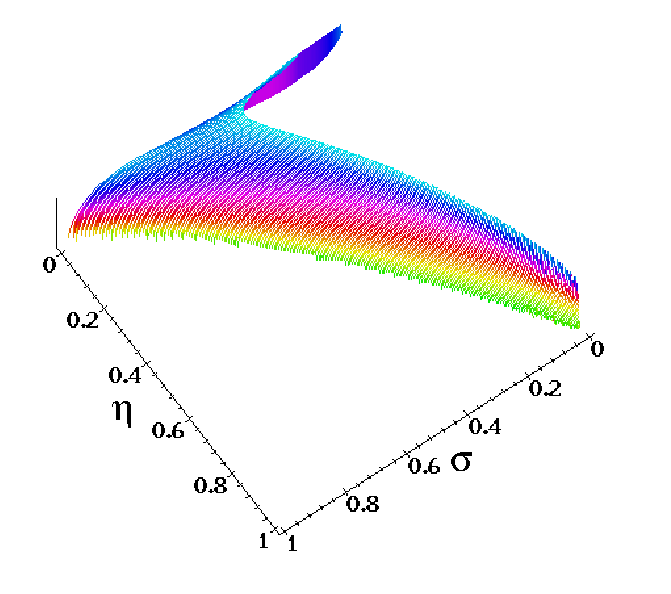
\epsfig{file=pics/surface.eps,width=10cm}
\caption{Amplitude~\eqref{ampli} des Lösungsansatzes~\eqref{ansatz} gezeigt
für  $A\in[0\ldots0.7]$ (zur besseren Übersicht farbig kodiert).}
\label{surface}
\end{figure}

\subsection{Biologische Interpretation}
\label{biointerpret}

Die Analyse des elastischen Netzes in Abschnitt~\ref{stabilitaet} hat
gezeigt, daß für fest gewählte Modellparameter $\sigma$ und $\eta$
kolumnäre Strukturen nur entstehen, wenn~$\sigma$ kleiner ist als ein
kritischer Wert $\sigma_i^\ast$.  Die Dynamik~\eqref{endyn} des elastischen
Netzes beschreibt ein Wechselspiel zwischen ``Konkurrenz'' und
``Kooperation''.  Jede Konfiguration der Merkmalsvektoren $\mathbf{R(x)}$
ist daher ein Kompromiß zwischen diesen beiden ``Kräften'': Der
Wettbewerb der Neurone $\mathbf{x}$ um die Reize $\mathbf{S}$ treibt diese
dazu, verschiedene rezeptive Felder $\mathbf{R(x)}$ zu entwickeln. Die
Kooperation zwischen benachbarten Neuronen dagegen gleicht deren rezeptiven
Feldeigenschaften tendentiell einander an.  Die Linie im Phasendiagram
(Abb.~\ref{spektrum}b) trennt die Gebiete in denen die Kooperation
bzw. die Konkurrenz dominiert. Kooperation und Konkurrenz halten sich auf
dieser Linie die Waage. Für gegebenes $\sigma_i$ ist die Wellenlänge
$\Lambda_i$ der emergierenden kolumnären Muster bestimmt durch

\begin{equation}
\Lambda_i = \frac{2 \pi}{\sqrt{\ln\left(\left<S_i^2\right>/\eta\right)}}\;\sigma_i
\label{lambda}
\end{equation}

Dieser Zusammenhang erlaubt es, die in biologischen Systemen nicht
meßbaren Varianzen $\left<S_i^2\right>$ durch Vorgabe der Observablen
$\Lambda_i$ sinnvoll einzustellen.  Gleichung~\eqref{lambda} hat eine
anschauliche, biologische Bedeutung: die Wellenlänge einer kolumnären
Struktur ist proportional zur typischen Größe eines, durch einen Stimulus
hervorgerufenen Erregungsgebietes. Neurone innerhalb eines solchen Gebietes
sind gleichzeitig aktiv, und haben daher die Tendenz, ähnliche Spezifität
zu entwickeln. Die Erregungsgebiete wirken als ``Saatkörner'' der
kolumnären Strukturen.
